\documentclass[11pt]{article}
\usepackage{graphicx}
\usepackage{enumitem}
\usepackage{csquotes}
\usepackage[hidelinks]{hyperref}
\usepackage[spanish]{babel}
\usepackage{tikz}
\usepackage{float}
\usepackage{xcolor}
\usepackage{amsmath}
\usepackage{cleveref}
\usepackage{subcaption}
\usepackage[style = apa, backend = biber, sorting = nty]{biblatex}
\usepackage[top=2.5cm, bottom=3cm, left=2.5cm, right=2cm]{geometry}

\addbibresource{bibliografia.bib}
\begin{document}

\nocite{usclogo}
\begin{titlepage}
\definecolor{AzulUSC}{RGB}{0,68,140}
\begin{tikzpicture}[remember picture,overlay]

\fill[AzulUSC!70!black] (current page.north west) rectangle 
    ([xshift=4cm]current page.south west);

\node[anchor=north east] at ([xshift=-2cm,yshift=-2cm]current page.north east) 
    {
\includegraphics[width=6cm]{USClogo.png}};
\end{tikzpicture}

\vspace*{5cm}
\begin{center}
    {\Huge \textbf{Memoria de Laboratorio}}\\[0.75cm]
    {\Large Instrumentación Electrónica}\\ [0.25cm]
    {\Large Corriente Continua y Alterna}\\[2cm]
    {\Large Pablo Méndez Fresco}\\[0.5cm]
    {\large Febrero 2026}
\end{center}
\end{titlepage}

\renewcommand{\listtablename}{Índice de tablas}
\renewcommand{\tablename}{Tabla}

\tableofcontents
\listoffigures
\listoftables
\newpage

\section{Práctica I (Corriente Continua)}
\subsection{\textbf{Objetivos}}
\begin{enumerate}%[label=\alph*)]
    \item Uso del polímetro (multímetro)
    \item Aplicación del código de colores para interpretar el valor de una resistencia
    \item Comprobación de la ley de Ohm y del cumplimiento de las leyes básicas de asociación de resistencias
\end{enumerate}

\subsection{\textbf{Materiales}}
\begin{enumerate}%[label=\alph*)]
    \item Placa base y cables de conexión
    \item Polímetro
    \item Resistencias (2)
    \item Fuente de alimentación de corriente continua
\end{enumerate}

\subsection{\textbf{Resistencias individuales}}
\subsubsection{Metodología}

\begin{itemize}
    \item Anotar el código de color de cada resistencia.
    \item Consultar la tabla para saber el valor dado por el fabricante.
    \item Utilizar el polímetro para obtener una medida directa de cada una de ellas.
    \item Utilizar nuevamente el polímetro, pero esta vez para el voltaje y la intensidad.
    \begin{itemize}
        \item Construir del circuito, como se muestra en la Fig \ref{fig:Resistenciaa}.
        \item Encender la fuente y fijar un voltaje para ambas mediciones.
        \item Medir el voltaje conectando cada 'cocodrilo' a un borne distinto de la resistencia.
        \item Medir la intensidad, prestando especial atención a la colocación del polímetro, 
        es decir, el polímetro debe cerrar el circuito.
    \end{itemize}
    \item Estimar mediante una recta de regresión la resistencia ($Ley$ $de$ $Ohm$).
\end{itemize}

\subsubsection{Discusión}

Para el transcurso de la práctica dispusimos de dos resistencias, la primera de ellas con un código de colores
Rojo-Rojo-Amarillo-Dorado y la segunda Amarillo-Violeta-Amarillo-Dorado, cuyas equivalencias numericas se 
recogen en la Tabla \ref{tab:Resistencias}.

\begin{table}[H]
\centering
\begin{tabular}{|c|c|c|c|}
\hline
Resistencia & Valor nominal ($\Omega$) & Tolerancia(\%) & $R \pm s(R) \hspace{4pt} (\Omega)$ \\
\hline
$R_1$ & $2,2\cdot 10^5$ & $\pm 5 \% $& $(2,2 \pm 0,11)\cdot 10^5$\\
$R_2$ & $4,7\cdot 10^5$ & $\pm 5 \% $ & $(4,7 \pm 0,23)\cdot 10^5$\\
\hline
\end{tabular}
\caption{Valores de las resistencias especificadas por el fabricante}
\label{tab:Resistencias}
\end{table}

A continuación, conectamos el polímetro a los bornes de cada resistencia de forma individual,
de tal forma que obtuvimos los resultados mostrados en la Tabla \ref{tab:R1}.

\begin{table}[H]
\centering
\begin{tabular}{|c|c|c|c|}
\hline
Resistencia & Lectura ($\Omega$) & Resolución ($\Omega$) & $R \pm s(R) \hspace{4pt} (\Omega)$\\
\hline
$R_1$ & $2,18\cdot 10^5$ & $\pm 10^3 $ & $(2,18 \pm 0,01) \cdot 10^5$\\
$R_2$ & $4,74\cdot 10^5$ & $\pm 10^3 $ & $(4,74 \pm 0,01) \cdot 10^5$\\
\hline
\end{tabular}
\caption{Valores de las resistencias medidos con el polímetro}
\label{tab:R1}
\end{table}

En cuanto a la estimación indirecta de la $R_1$, procedimos según se indica en la metodología. Nuestro objetivo es observar
la relación lineal que hay entre el voltaje y la intensidad de $R_1$, donde esta viene dada por la $Ley$ $de$ $Ohm:$
\begin{equation}
    V = I \cdot R \Rightarrow R = \frac{V}{I} 
\end{equation}

\begin{table}[H]
\centering
\begin{tabular}{|c|c|c|}
\hline
Medidas & $V \pm s(V) \hspace{4pt} (V)$ & $I \pm s(I) \hspace{4pt} (A)$ \\
\hline
1 & $(1,068 \pm 0,001)$ & $(4,8 \pm 0,1) \cdot 10^{-6}$ \\
2 & $(2,05 \pm 0,01)$ & $(9,3 \pm 0,1) \cdot 10^{-6}$ \\
3 & $(3,06 \pm 0,01)$ & $(1,39 \pm 0,01) \cdot 10^{-5}$ \\
4 & $(4,04 \pm 0,01)$ & $(1,84 \pm 0,01) \cdot 10^{-5}$ \\
5 & $(5,06 \pm 0,01)$ & $(2,30 \pm 0,01) \cdot 10^{-5}$ \\
6 & $(6,07 \pm 0,01)$ & $(2,77 \pm 0,01) \cdot 10^{-5}$ \\
7 & $(7,06 \pm 0,01)$ & $(3,22 \pm 0,01) \cdot 10^{-5}$ \\
8 & $(8,04 \pm 0,01)$ & $(3,66 \pm 0,01) \cdot 10^{-5}$ \\
9 & $(9,03 \pm 0,01)$ & $(4,12 \pm 0,01) \cdot 10^{-5}$ \\
10 & $(10,04 \pm 0,01)$ & $(4,57 \pm 0,01) \cdot 10^{-5}$ \\
11 & $(11,06 \pm 0,01)$ & $(5,04 \pm 0,01) \cdot 10^{-5}$ \\
\hline
\end{tabular}
\caption{Potenciales e intensidades para el circuito simple con la resistencia $R_1$ (Fig. \ref{fig:Resistenciaa})}
\label{tab:Resistencias2}
\end{table}

De los datos podemos realizar las siguientes operaciones (\ref{eq:sumx}) 
con el fin de minimizar el ECM de la recta de regresión, seguido de los cálculos de los dos parametros de la 
recta de regresión simple y su incertidumbre (\ref{eq:a1}),(\ref{eq:b1}),(\ref{eq:s1}),(\ref{eq:s1a}),(\ref{eq:s1b});
la incertidumbre y los coeficientes $R$ y $R^2$ que indican la calidad del ajuste (\ref{eq:R1}),(\ref{eq:R12}) :

\begin{center}
\begin{equation}
\begin{split}
    \sum^n_{i=1} x_i = 3,032 \hspace{3pt}[V] \hspace{20pt}
    \sum^n_{i=1} y_i = 66,578 \cdot 10^{-4} \hspace{3pt}[A]\hspace{20pt}
    \sum^n_{i=1} x_i^2 = 1,064008 \cdot 10^{-8} \hspace{3pt} [V^2] \hspace{20pt} \\
    \sum^n_{i=1} x_i y_i = 2,3354644 \cdot 10^{-3} \hspace{3pt} [V\cdot A] \hspace{20pt}
    \sum^n_{i=1} y_i^2 = 512,628124 \hspace{3pt}[A^2] \hspace{20pt}
    n=11\hspace{20pt}
    \label{eq:sumx}
\end{split}
\end{equation}
\end{center}

\begin{center}
\begin{align}
    a = \frac{(\sum^n_{i=1} y_i)(\sum^n_{i=1} x^2_i )-(\sum^n_{i=1} x_i)(\sum^n_{i=1} x_i y_i)}{n(\sum^n_{i=1} x_i^2)-(\sum^n_{i=1} x_i)^2} &\Rightarrow a= 0,0112\hspace{6pt} [V] \label{eq:a1}\\
    b = \frac{n(\sum^n_{i=1} x_i y_i)-(\sum^n_{i=1} x_i)(\sum^n_{i=1} y_i)}{n(\sum^n_{i=1} x_i^2)-(\sum^n_{i=1} x_i)^2} &\Rightarrow b= 219180 \hspace{6pt}[\Omega] \label{eq:b1}\\
    s_{y|x} =\sqrt\frac{\sum^n_{i=1}(y_i-(a+b x_i))^2}{n-2} &\Rightarrow s_{y|x}= 0,0086 \hspace{6pt}[V] \label{eq:s1}\\
    s(a) =s_{y|x} \cdot \sqrt\frac{\sum^n_{i=1}x_i^2}{n(\sum^n_{i=1} x_i^2)-(\sum^n_{i=1} x_i)^2} &\Rightarrow s(a)= 0,0056 \hspace{6pt}[V] \label{eq:s1a}\\
    s(b) =s_{y|x} \cdot \sqrt\frac{n}{n(\sum^n_{i=1} x_i^2)-(\sum^n_{i=1} x_i)^2} &\Rightarrow s(b) = 180 \hspace{6pt}[\Omega] \label{eq:s1b}\\
    r = \frac{n(\sum^n_{i=1} x_i y_i)-(\sum^n_{i=1} x_i)(\sum^n_{i=1} y_i)}{\sqrt{[n(\sum^n_{i=1} x_i^2)-(\sum^n_{i=1} x_i)^2][n(\sum^n_{i=1} y_i^2)-(\sum^n_{i=1} y_i)^2]}}&\Rightarrow r= 0,999996 \label{eq:R1}\\
    R^2 =r^2&\Rightarrow R^2=0.999993 \label{eq:R12}
\end{align}
\end{center}


Quedando la mejor recta con la forma:

\begin{equation}
    \hat{y}= (0,0112 \pm 0,0056)\hspace{3pt}+ \hspace{3pt}(219180 \pm 180)x \hspace{6pt} [V]
\end{equation}

\begin{figure}[H]
    \begin{center}
        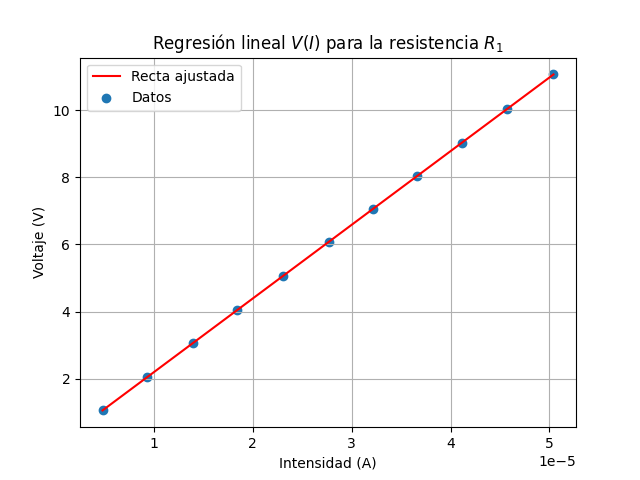
\includegraphics[width=14cm]{Figure_1M1.png}
    \end{center}
    \caption{Regresión lineal $V(I)$ para la resistencia $R_1$}
\end{figure}

\subsubsection{Resultados}
\label{sec:1.3}

A la luz de las tablas y de la experimentación previamente expuesta, se puede concluir que para $R_1$ la resistividad medida
con el polímetro, así como sus ramas, caen dentro del intervalo de confianza delimitado por el fabricante (Para $k\leq1$), pues 
$(2,18 \pm 0,01) \cdot 10^5 \subset ((2,2 - 0,11)\cdot 10^5;(2,2 + 0,11)\cdot 10^5)$. 

\medskip

Por otra parte, la recta de regresión de V-I 
se ajusta con un $R^2$ muy próximo a $1$, lo que indica que los datos son casi lineales. La justificación de esta discrepancia es el 
error que puede llevar cada medida, así como la presencia de un entorno que puede cambiar y alterar cada medida (Errores aleatorios).
Además, durante todas las mediciones se observó que el polímetro presentaba un error sistematico al medir voltaje, ya que al conectarlo a la
fuente de alimentacion con $0V$ este indicaba valores en un intervalo $[0,03;0,04] \hspace{4pt}V$. Con todo, $b=219176,3651$ 
implica una diferencia de menos de $1 \hspace{4pt} k\Omega$ con la media del valor ofrecido por el fabricante y una diferencia 
similar con el medido expermentalmente, en ambos casos dentro del intervalo de confianza que aporta $s(b)$ 
(Con $k=2$ para la medida experimental) con una confianza superior al 99\%; 
y $a=0,0112$ implica que la recta no pasa por el origen, pero de nuevo, esto se debe, probablemente, a errores aleatorios y al 
bajo número de datos.

\subsection{\textbf{Circuito Serie}}
\subsubsection{Metodología}

\begin{itemize}
    \item Estimación teórica de las resistencias en serie y la resistencia total equivalente mediante
    la $Ley$ $de$ $Ohm$ y la propagación de incertidumbres.
    \item Construcción del circuito en serie Fig \ref{fig:Seriee}
    \item Estimación directa de la $R_T$ mediante uso del polímetro, colocado al principio y al final del circuito 
    \item Utilizar nuevamente el polímetro, pero esta vez para la intensidad y los voltajes totales, de $R_1$ y $R_2$.
    \begin{itemize}
        \item Encender la fuente y fijar un voltaje para ambas mediciones.
        \item Medir el voltaje conectando cada 'cocodrilo' a un borne distinto de cada resistencia.
        \item Medir el voltaje conectando cada 'cocodrilo' a un borne de cada resistencia de tal forma que quede en paralelo a ambas resistencias.
        \item Medir la intensidad, prestando especial atención a la colocación del polímetro, 
        es decir, el polímetro debe cerrar el circuito (se usará la $Ley$ $de$ $Ohm$ para no medir $I_1$ e $I_2$).
    \end{itemize}
    \item Estimar mediante una recta de regresión la resistencia ($Ley$ $de$ $Ohm$).
    \item Estimar mediante suma y propagación de errores la suma de los voltajes $V_1$ y $V_2$ con $V_T$.
\end{itemize}

\subsubsection{Discusión}

Primero se realizará el cálculo teórico de la resistencia equivalente de acuerdo con (\ref{eq:qwer}):
\begin{equation}
\begin{split}
    R_{S_T}=\sum^n_i R_i  \Rightarrow R_{S_T} = R_1 + R_2 = 2,2 \cdot 10^5 + 4,7 \cdot 10^5 = 6,9 \cdot 10^5 \hspace{4pt}[\Omega] \\
    u(R_{S_T})=\sqrt{\sum^n_{i=1} \left( \frac{\partial R_S}{\partial R_i} \right)^2\hspace{2 pt} s^2(R_i)}=\sqrt{s(R_1)^2+s(R_2)^2}
    =0,25947 \cdot 10^5 \hspace{4pt}[\Omega] \\
    R_{S_T} \pm s(R_{S_T})=(6,9 \pm 0,25947)\cdot 10^5 \hspace{4pt}[\Omega]
    \label{eq:qwer}
\end{split}
\end{equation}

A continuación, medimos la resistencia total equivalente del circuito en serie con el polímetro, es decir, colocando un borne
al principio de $R_1$ y otro tras $R_2$. Obtuvimos lo siguiente (\ref{eq:tre}):

\begin{equation}
    R_{S_e} \pm s(R_{S_e}) = (6,93 \pm 0,01) \cdot 10^5 \hspace{4pt} [\Omega]
    \label{eq:tre}
\end{equation}

En cuanto a las medidas indirectas, antes de nada se comprobará que la ecuación (\ref{eq:voltajes}) se verifica, representandolo
en Tabla \ref{tab:Serie2}:

\begin{equation}
\begin{split}
    V_S= \epsilon_S = V_1 + V_2 \hspace{4pt} [V] \\
    u(V_S)=\sqrt{\sum^n_{i=1} \left( \frac{\partial V_S}{\partial V_i} \right)^2\hspace{2 pt} s^2(V_i)}=\sqrt{s(V_1)^2+s(V_2)^2}
     \hspace{4pt}[V]
    \label{eq:voltajes}
\end{split}
\end{equation}

\begin{table}[ht]
\centering
\begin{tabular}{|c|c|c|c|c|}
\hline
Medidas &$V \pm s(V)\hspace{4pt}(V)$&$V_1 \pm s(V_1)\hspace{4pt}(V)$&$V_2 \pm s(V_2)\hspace{4pt}(V)$&$V_S\pm u(V_S)\hspace{4pt}(V)$\\
\hline
1 & $(1,034 \pm 0,001)$ &$(0,321 \pm 0,001)$& $(0,698 \pm 0,001)$ &($1,0190\pm 0,0014)$\\
2 & $(2,06 \pm 0,01)$ &$(0,641 \pm 0,001)$& $(1,392 \pm 0,001)$ &($2,0330\pm 0,0014$) \\
3 & $(3,03 \pm 0,01)$ &$(0,943 \pm 0,001)$& $(2,04 \pm 0,01)$ &($2,983\pm 0,01$) \\
4 & $(4,03 \pm 0,01)$ &$(1,253 \pm 0,001)$& $(2,72 \pm 0,01)$ & ($3,973 \pm 0,01$) \\
5 & $(5,07 \pm 0,01)$ &$(1,575 \pm 0,001)$& $(3,42 \pm 0,01)$ &($4,995 \pm 0,01$) \\
6 & $(6,04 \pm 0,01)$ &$(1,87 \pm 0,01)$& $(4,07 \pm 0,01)$ & ($5,940 \pm 0,014$) \\
7 & $(7,07 \pm 0,01)$ &$(2,19 \pm 0,01)$& $(4,76 \pm 0,01)$ & ($6,950 \pm 0,014$)\\
8 & $(8,07 \pm 0,01)$ &$(2,51 \pm 0,01)$& $(5,44 \pm 0,01)$ &($7,950\pm 0,014$) \\
9 & $(9,04 \pm 0,01)$ &$(2,80 \pm 0,01)$& $(6,09 \pm 0,01)$ &($8,890\pm 0,014$) \\
10 & $(10,05 \pm 0,01)$ &$(3,12 \pm 0,01)$& $(6,78 \pm 0,01)$ & ($9,900\pm 0,014$)\\
11 & $(11,09 \pm 0,01)$ &$(3,44 \pm 0,01)$& $(7,47 \pm 0,01)$ & ($10,91 \pm 0,014$)\\
\hline
\end{tabular}
\caption{Potenciales del circuito en serie y cálculo de (Ec. \ref{eq:voltajes})}
\label{tab:Serie2}
\end{table}

Tras esto, se siguieron los pasos de la metodología para obtener once datos tal y como se recogen en la Tabla \ref{tab:Serie}:

\begin{table}[H]
\centering
\begin{tabular}{|c|c|c|c|c|}
\hline
Medidas &$V \pm s(V)\hspace{4pt}(V)$&$V_1 \pm s(V_1)\hspace{4pt}(V)$&$V_2 \pm s(V_2)\hspace{4pt}(V)$&$I \pm s(I)\hspace{4pt}(A)$\\
\hline
1 & $(1,034 \pm 0,001)$ &$(0,321 \pm 0,001)$& $(0,698 \pm 0,001)$ & $(1,4 \pm 0,1) \cdot 10^{-6}$ \\
2 & $(2,06 \pm 0,01)$ &$(0,641 \pm 0,001)$& $(1,392 \pm 0,001)$ & $(2,9 \pm 0,1) \cdot 10^{-6}$ \\
3 & $(3,03 \pm 0,01)$ &$(0,943 \pm 0,001)$& $(2,04 \pm 0,01)$ & $(4,3 \pm 0,1) \cdot 10^{-6}$ \\
4 & $(4,03 \pm 0,01)$ &$(1,253 \pm 0,001)$& $(2,72 \pm 0,01)$ & $(5,7 \pm 0,1) \cdot 10^{-6}$ \\
5 & $(5,07 \pm 0,01)$ &$(1,575 \pm 0,001)$& $(3,42 \pm 0,01)$ & $(7,2 \pm 0,1) \cdot 10^{-6}$ \\
6 & $(6,04 \pm 0,01)$ &$(1,87 \pm 0,01)$& $(4,07 \pm 0,01)$ & $(8,6 \pm 0,1) \cdot 10^{-6}$ \\
7 & $(7,07 \pm 0,01)$ &$(2,19 \pm 0,01)$& $(4,76 \pm 0,01)$ & $(1,01 \pm 0,01) \cdot 10^{-5}$ \\
8 & $(8,07 \pm 0,01)$ &$(2,51 \pm 0,01)$& $(5,44 \pm 0,01)$ & $(1,15 \pm 0,01) \cdot 10^{-5}$ \\
9 & $(9,04 \pm 0,01)$ &$(2,80 \pm 0,01)$& $(6,09 \pm 0,01)$ & $(1,29 \pm 0,01) \cdot 10^{-5}$ \\
10 & $(10,05 \pm 0,01)$ &$(3,12 \pm 0,01)$& $(6,78 \pm 0,01)$ & $(1,44 \pm 0,01) \cdot 10^{-5}$ \\
11 & $(11,09 \pm 0,01)$ &$(3,44 \pm 0,01)$& $(7,47 \pm 0,01)$ & $(1,59 \pm 0,01) \cdot 10^{-5}$ \\
\hline
\end{tabular}
\caption{Potenciales e intensidades para el circuito en serie (Fig. \ref{fig:Seriee})}
\label{tab:Serie}
\end{table}

De los datos podemos realizar las siguientes operaciones (\ref{eq:sumx2}) 
con el fin de minimizar el ECM de la recta de regresión, seguido de los cálculos de los dos parametros de la 
recta de regresión simple y su incertidumbre (\ref{eq:a2}),(\ref{eq:b2}),(\ref{eq:s2}),(\ref{eq:s2a}),(\ref{eq:s2b});
la incertidumbre y los coeficientes $R$ y $R^2$ que indican la calidad del ajuste (\ref{eq:R2}),(\ref{eq:R22}) :

\begin{equation}
\begin{split}
    \sum^n_{i=1} x_i = 9,49 \cdot 10^{-3} \hspace{3pt}[V] \hspace{20pt}
    \sum^n_{i=1} y_i = 66,584 \hspace{3pt}[A]\hspace{20pt}
    \sum^n_{i=1} x_i^2 = 1,04799 \cdot 10^{-9}\hspace{3pt} [V^2] \hspace{20pt} \\
    \sum^n_{i=1} x_i y_i = 7,337486 \cdot 10^{-3} \hspace{3pt} [V\cdot A] \hspace{20pt}
    \sum^n_{i=1} y_i^2 = 513,743056 \hspace{3pt}[A^2] \hspace{20pt}
    n=11\hspace{20pt}
    \label{eq:sumx2}
\end{split}
\end{equation}
\bigskip
\begin{center}
\begin{align}
    a = \frac{(\sum^n_{i=1} y_i)(\sum^n_{i=1} x^2_i )-(\sum^n_{i=1} x_i)(\sum^n_{i=1} x_i y_i)}{n(\sum^n_{i=1} x_i^2)-(\sum^n_{i=1} x_i)^2} &\Rightarrow a= 0,0581\hspace{6pt} [V] \label{eq:a2}\\
    b = \frac{n(\sum^n_{i=1} x_i y_i)-(\sum^n_{i=1} x_i)(\sum^n_{i=1} y_i)}{n(\sum^n_{i=1} x_i^2)-(\sum^n_{i=1} x_i)^2} &\Rightarrow b= 694880 \hspace{6pt}[\Omega] \label{eq:b2}\\
    s_{y|x} =\sqrt\frac{\sum^n_{i=1}(y_i-(a+b x_i))^2}{n-2} &\Rightarrow s_{y|x}= 0,0148 \hspace{6pt}[V] \label{eq:s2}\\
    s(a) =s_{y|x} \cdot \sqrt\frac{\sum^n_{i=1}x_i^2}{n(\sum^n_{i=1} x_i^2)-(\sum^n_{i=1} x_i)^2} &\Rightarrow s(a)= 0,0095 \hspace{6pt}[V] \label{eq:s2a}\\
    s(b) =s_{y|x} \cdot \sqrt\frac{n}{n(\sum^n_{i=1} x_i^2)-(\sum^n_{i=1} x_i)^2} &\Rightarrow s(b)= 970 \hspace{6pt}[\Omega] \label{eq:s2b}\\
    r = \frac{n(\sum^n_{i=1} x_i y_i)-(\sum^n_{i=1} x_i)(\sum^n_{i=1} y_i)}{\sqrt{[n(\sum^n_{i=1} x_i^2)-(\sum^n_{i=1} x_i)^2][n(\sum^n_{i=1} y_i^2)-(\sum^n_{i=1} y_i)^2]}}&\Rightarrow r= 0,999991 \label{eq:R2}\\
    R^2 =r^2&\Rightarrow R^2=0.99998 \label{eq:R22}
\end{align}
\end{center}

Quedando la mejor recta con la forma:

\begin{equation}
    \hat{y}= (0,0581 \pm 0,0095) \hspace{3pt} + \hspace{3pt}(694880 \pm 970)x\hspace{6pt} [V]
\end{equation}

\begin{figure}[H]
    \begin{center}
        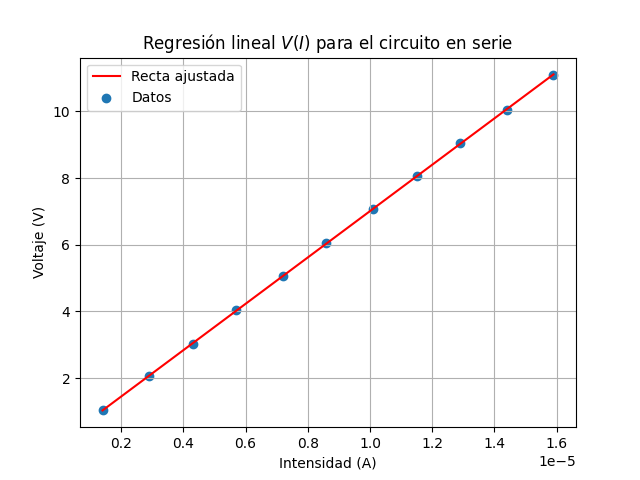
\includegraphics[width=14cm]{Figure_2M1.png}
    \end{center}
    \caption{Regresión lineal $V(I)$ del circuito en serie}
\end{figure}


\subsubsection{Resultados}
\label{sec:1.4}

Podemos concluir que la medición experimental cae de lleno en el intervalo  dado por la $Ley$ $de$ $Ohm$ 
y la propagación de errores (\ref{eq:qwer}) $[(6,93 \pm 0,01) \cdot 10^5 \subset ((6,9 - 0,25947)\cdot 10^5,(6,9 + 0,25947)\cdot 10^5)]$.
En lo que respecta a la verificación de (\ref{eq:voltajes}), observamos que la suma siempre es menor que el valor medido con el polímetro.
Dos posibles explicaciones son la propia resistividad de los cables, que tomamos como nula a lo largo de toda la práctica, y la otra son los
errores aleatorios en el transcurso de las medidas. 

\medskip

La mejor recta se ajusta con un $R^2 = 0,9998 \approx 1$,entonces podemos concluir que los datos siguen una distribución lineal de parámetros
$a$ y $b$.
Respecto a la recta de regresión en sí, se observa otra vez el error de la coordenada en el origen $(a\neq 0)$ es en gran parte por el error
sistemático del polímetro, el cual oscilaba en torno a $0,04 \hspace{4pt}[V]$.
En cuanto a la pendiente de la recta, $b=694883,579\hspace{6pt}[\Omega]$
está también en el intervalo teórico; y en específico, se aproxima mucho más al medido por el polímetro $(R_{S_e})$, apreciando
una discrepancia similar a la de la Sección \ref{sec:1.3}.

\subsection{\textbf{Circuito Paralelo}}
\subsubsection{Metodología}

\begin{itemize}
    \item Estimación teórica de las resistencias en paralelo y la resistencia total equivalente mediante
    la $Ley$ $de$ $Ohm$ y la propagación de incertidumbres.
    \item Construcción del circuito en serie Fig \ref{fig:Paraleloo}
    \item Estimación directa de la $R_T$ mediante uso del polímetro, colocado al principio y al final del circuito 
    \item Utilizar nuevamente el polímetro, pero esta vez para el potencial y las intensidades totales, de $R_1$ y $R_2$.
    \begin{itemize}
        \item Encender la fuente y fijar un voltaje para ambas mediciones.
        \item Medir la intensidad total cerrando el circuito con ambos 'cocodrilos' sin que estos estén en paralelo con ningún componente.
        \item Medir las intensidades individuales conectando un 'cocodrilo' a un borne de una resistencia de tal forma que toda la corriente
        fluya por el amperímetro.
        \item Medir el voltaje de todo el circuito conectando un borne previo a $R_1$ y otro tras $R_2$  
        (Se usará la $Ley$ $de$ $Ohm$ para no medir $V_1$ e $V_2$).
    \end{itemize}
    \item Estimar mediante una recta de regresión la resistencia ($Ley$ $de$ $Ohm$).
    \item Estimar mediante suma y propagación de errores la suma de las intensidades $I_1$ y $I_2$ con $I_T$.
\end{itemize}

\subsubsection{Discusión}

Primero se realizará el cálculo teórico de la resistencia equivalente de acuerdo con (\ref{eq:qwertr}):
\begin{center}
\begin{equation}
\begin{split}
    \frac{1}{R_{P_T}}=\sum^n_{i=1} \frac{1}{R_i}  \Rightarrow \frac{1}{R_{P_T}} = \frac{R_1 + R_2}{R_1 \cdot R_2} = \frac{2,2 \cdot 10^5 + 4,7 \cdot 10^5}
    {2,2 \cdot 10^5 \cdot 4,7 \cdot 10^5} \Rightarrow R_{P_T}= 1,498550725 \cdot 10^5 \hspace{4pt}[\Omega] \\
    \medskip
    u(R_{P_T})=\sqrt{\sum^n_{i=1} \left( \frac{\partial R_P}{\partial R_i} \right)^2\hspace{2 pt} s^2(R_i)}
    =\sqrt{\sum^n_{i=1} \left( \frac{\partial}{\partial R_i}\left[\left(\frac{1}{R_1}+\frac{1}{R_2}\right)^{-1}\right] \right)^2\hspace{2 pt}
    s^2(R_i)}=\\ 
    \medskip
    =\sqrt{\sum^n_{i=1} \left( \frac{\partial}{\partial R_i}\left[\frac{R_1 \cdot R_2}{R_1+R_2}\right] \right)^2\hspace{2 pt} s^2(R_i)}=%\\
    \sqrt{\frac{1}{(R_1+R_2)^4} \cdot \left(R_2^4 \hspace{2 pt}s^2(R_1) + R_1^4 \hspace{2 pt}s^2(R_2)\right)}
    =0,0563521 \cdot 10^5 \hspace{4pt}[\Omega] \\
    \bigskip
    R_{P_T} \pm u(R_{P_T})=(1,499 \pm 0,056)\cdot 10^5 \hspace{4pt}[\Omega]
    \label{eq:qwertr}
\end{split}
\end{equation}
\end{center}

A continuación, medimos la resistencia total equivalente del circuito en serie con el polímetro, es decir, colocando un borne
al principio de $R_1$ y otro tras $R_2$. Obtuvimos lo siguiente (\ref{eq:trer}):

\begin{equation}
    R_{P_e} \pm s(R_{P_e}) = (1,495 \pm 0,001) \cdot 10^5 \hspace{4pt} [\Omega]
    \label{eq:trer}
\end{equation}

En cuanto a las medidas indirectas, antes de nada se comprobará que la ecuación (\ref{eq:intensidades}) se verifica, representandolo
en Tabla \ref{tab:intensidades}:

\begin{equation}
\begin{split}
    I_P= I_1 + I_2 \hspace{4pt} [A] \\
    u(I_P)=\sqrt{\sum^n_{i=1} \left( \frac{\partial I_P}{\partial I_i} \right)^2\hspace{2 pt} s^2(I_i)}=\sqrt{s(I_1)^2+s(I_2)^2}
     \hspace{4pt}[V]
    \label{eq:intensidades}
\end{split}
\end{equation}

\begin{table}[H]
\centering
\begin{tabular}{|c|c|c|c|c|}
\hline
Med. & $I \pm s(I)\hspace{4pt}(A)$ & $I_1 \pm s(I_1)\hspace{4pt}(A)$ & $I_2 \pm s(I_2)\hspace{4pt}(A)$ & $I_P \pm u(I_P)\hspace{4pt}(A)$ \\
\hline
1 & $(6,9 \pm 0,1) \cdot 10^{-6}$ & $(4,7 \pm 0,1) \cdot 10^{-6}$ & $(2,1 \pm 0,1) \cdot 10^{-6}$ &  $(6,80 \pm 0,14) \cdot 10^{-6}$\\
2 & $(1,34 \pm 0,01) \cdot 10^{-5}$ & $(9,2 \pm 0,1) \cdot 10^{-6}$ & $(4,2 \pm 0,1) \cdot 10^{-6}$ &  $(1,340 \pm 0,014) \cdot 10^{-5}$\\
3 & $(2,01 \pm 0,01) \cdot 10^{-5}$ & $(1,37 \pm 0,01) \cdot 10^{-5}$ & $(6,3 \pm 0,1) \cdot 10^{-6}$ &  $(2,000 \pm 0,014) \cdot 10^{-5}$\\
4 & $(2,70 \pm 0,01) \cdot 10^{-5}$ & $(1,84 \pm 0,01) \cdot 10^{-5}$ & $(8,5 \pm 0,1) \cdot 10^{-6}$ &$(2,690 \pm 0,014) \cdot 10^{-5}$\\
5 & $(3,35 \pm 0,01) \cdot 10^{-5}$ & $(2,29 \pm 0,01) \cdot 10^{-5}$ & $(1,05 \pm 0,01) \cdot 10^{-5}$ &$(3,340 \pm 0,014) \cdot 10^{-5}$\\
6 & $(4,02 \pm 0,01) \cdot 10^{-5}$ & $(2,75 \pm 0,01) \cdot 10^{-5}$ & $(1,27 \pm 0,01) \cdot 10^{-5}$ & $(4,020 \pm 0,014) \cdot 10^{-5}$\\
7 & $(4,68 \pm 0,01) \cdot 10^{-5}$ & $(3,21 \pm 0,01) \cdot 10^{-5}$ & $(1,48 \pm 0,01) \cdot 10^{-5}$ & $(4,690 \pm 0,014) \cdot 10^{-5}$\\
8 & $(5,37 \pm 0,01) \cdot 10^{-5}$ & $(3,67 \pm 0,01) \cdot 10^{-5}$ & $(1,69 \pm 0,01) \cdot 10^{-5}$ & $(5,360 \pm 0,014) \cdot 10^{-5}$\\
9 & $(6,02 \pm 0,01) \cdot 10^{-5}$ & $(4,12 \pm 0,01) \cdot 10^{-5}$ & $(1,90 \pm 0,01) \cdot 10^{-5}$ & $(6,020 \pm 0,014) \cdot 10^{-5}$\\
10 & $(6,69 \pm 0,01) \cdot 10^{-5}$ & $(4,58 \pm 0,01) \cdot 10^{-5}$ & $(2,11 \pm 0,01) \cdot 10^{-5}$ & $(6,690 \pm 0,014) \cdot 10^{-5}$\\
11 & $(7,36 \pm 0,01) \cdot 10^{-5}$ & $(5,04 \pm 0,01) \cdot 10^{-5}$ & $(2,32 \pm 0,01) \cdot 10^{-5}$ & $(7,360 \pm 0,014) \cdot 10^{-5}$\\
\hline
\end{tabular}
\caption{Intensidades del circuito en paralelo y cálculo de (Ec. \ref{eq:intensidades})}
\label{tab:intensidades}
\end{table}

A continuación, se siguieron los pasos de la metodología para obtener los siguientes datos tal y como se recogen en la Tabla \ref{tab:Paralelo}:

\begin{table}[H]
\centering
\begin{tabular}{|c|c|c|c|c|}
\hline
Medidas & $V \pm s(V)\hspace{4pt}(V)$ & $I_1 \pm s(I_1)\hspace{4pt}(A)$ & $I_2 \pm s(I_2)\hspace{4pt}(A)$ & $I \pm s(I)\hspace{4pt}(A)$ \\
\hline
1 & $(1,041 \pm 0,001)$ & $(4,7 \pm 0,1) \cdot 10^{-6}$ & $(2,1 \pm 0,1) \cdot 10^{-6}$ & $(6,9 \pm 0,1) \cdot 10^{-6}$ \\
2 & $(2,02 \pm 0,01)$ & $(9,2 \pm 0,1) \cdot 10^{-6}$ & $(4,2 \pm 0,1) \cdot 10^{-6}$ & $(1,34 \pm 0,01) \cdot 10^{-5}$ \\
3 & $(3,02 \pm 0,01)$ & $(1,37 \pm 0,01) \cdot 10^{-5}$ & $(6,3 \pm 0,1) \cdot 10^{-6}$ & $(2,01 \pm 0,01) \cdot 10^{-5}$ \\
4 & $(4,05 \pm 0,01)$ & $(1,84 \pm 0,01) \cdot 10^{-5}$ & $(8,5 \pm 0,1) \cdot 10^{-6}$ & $(2,70 \pm 0,01) \cdot 10^{-5}$ \\
5 & $(5,03 \pm 0,01)$ & $(2,29 \pm 0,01) \cdot 10^{-5}$ & $(1,05 \pm 0,01) \cdot 10^{-5}$ & $(3,35 \pm 0,01) \cdot 10^{-5}$ \\
6 & $(6,04 \pm 0,01)$ & $(2,75 \pm 0,01) \cdot 10^{-5}$ & $(1,27 \pm 0,01) \cdot 10^{-5}$ & $(4,02 \pm 0,01) \cdot 10^{-5}$ \\
7 & $(7,04 \pm 0,01)$ & $(3,21 \pm 0,01) \cdot 10^{-5}$ & $(1,48 \pm 0,01) \cdot 10^{-5}$ & $(4,68 \pm 0,01) \cdot 10^{-5}$ \\
8 & $(8,06 \pm 0,01)$ & $(3,67 \pm 0,01) \cdot 10^{-5}$ & $(1,69 \pm 0,01) \cdot 10^{-5}$ & $(5,37 \pm 0,01) \cdot 10^{-5}$ \\
9 & $(9,04 \pm 0,01)$ & $(4,12 \pm 0,01) \cdot 10^{-5}$ & $(1,90 \pm 0,01) \cdot 10^{-5}$ & $(6,02 \pm 0,01) \cdot 10^{-5}$ \\
10 & $(10,05 \pm 0,01)$ & $(4,58 \pm 0,01) \cdot 10^{-5}$ & $(2,11 \pm 0,01) \cdot 10^{-5}$ & $(6,69 \pm 0,01) \cdot 10^{-5}$ \\
11 & $(11,06 \pm 0,01)$ & $(5,04 \pm 0,01) \cdot 10^{-5}$ & $(2,32 \pm 0,01) \cdot 10^{-5}$ & $(7,36 \pm 0,01) \cdot 10^{-5}$ \\
\hline
\end{tabular}
\caption{Potenciales e intensidades para el circuito paralelo(Fig. \ref{fig:Paraleloo})}
\label{tab:Paralelo}
\end{table}

De los datos podemos realizar las siguientes operaciones (\ref{eq:sumx3}) 
con el fin de minimizar el ECM de la recta de regresión, seguido de los cálculos de los dos parametros de la 
recta de regresión simple y su incertidumbre (\ref{eq:a3}),(\ref{eq:b3}),(\ref{eq:s3}),(\ref{eq:s3a}),(\ref{eq:s3b});
la incertidumbre y los coeficientes $R$ y $R^2$ que indican la calidad del ajuste (\ref{eq:R3}),(\ref{eq:R32}) :

\begin{equation}
\begin{split}
    \sum^n_{i=1} x_i = 4,423 \cdot 10^{-4} \hspace{3pt}[V] \hspace{20pt}
    \sum^n_{i=1} y_i = 66,451 \hspace{3pt}[A]\hspace{20pt}
    \sum^n_{i=1} x_i^2 = 2,268901 \cdot 10^{-8}\hspace{3pt} [V^2] \hspace{20pt} \\
    \sum^n_{i=1} x_i y_i = 3,4084789 \cdot 10^{-3} \hspace{3pt} [V\cdot A] \hspace{20pt}
    \sum^n_{i=1} y_i^2 = 512,042381 \hspace{3pt}[A^2] \hspace{20pt}
    n=11\hspace{20pt}
    \label{eq:sumx3}
\end{split}
\end{equation}
\bigskip
\begin{center}
\begin{align}
    a = \frac{(\sum^n_{i=1} y_i)(\sum^n_{i=1} x^2_i )-(\sum^n_{i=1} x_i)(\sum^n_{i=1} x_i y_i)}{n(\sum^n_{i=1} x_i^2)-(\sum^n_{i=1} x_i)^2} &\Rightarrow a= 0,0025\hspace{6pt} [V] \label{eq:a3}\\
    b = \frac{n(\sum^n_{i=1} x_i y_i)-(\sum^n_{i=1} x_i)(\sum^n_{i=1} y_i)}{n(\sum^n_{i=1} x_i^2)-(\sum^n_{i=1} x_i)^2} &\Rightarrow b= 150176 \hspace{6pt}[\Omega] \label{eq:b3}\\
    s_{y|x} =\sqrt\frac{\sum^n_{i=1}(y_i-(a+b x_i))^2}{n-2} &\Rightarrow s_{y|x}= 0,0054 \hspace{6pt}[V] \label{eq:s3}\\
    s(a) =s_{y|x} \cdot \sqrt\frac{\sum^n_{i=1}x_i^2}{n(\sum^n_{i=1} x_i^2)-(\sum^n_{i=1} x_i)^2} &\Rightarrow s(a)= 0,0035 \hspace{6pt}[V] \label{eq:s3a}\\
    s(b) =s_{y|x} \cdot \sqrt\frac{n}{n(\sum^n_{i=1} x_i^2)-(\sum^n_{i=1} x_i)^2} &\Rightarrow s(b)= 77 \hspace{6pt}[\Omega] \label{eq:s3b}\\
    r = \frac{n(\sum^n_{i=1} x_i y_i)-(\sum^n_{i=1} x_i)(\sum^n_{i=1} y_i)}{\sqrt{[n(\sum^n_{i=1} x_i^2)-(\sum^n_{i=1} x_i)^2][n(\sum^n_{i=1} y_i^2)-(\sum^n_{i=1} y_i)^2]}}&\Rightarrow r= 0,999998 \label{eq:R3}\\
    R^2 =r^2&\Rightarrow R^2=0.999997 \label{eq:R32}
\end{align}
\end{center}

Quedando la mejor recta con la forma:

\begin{equation}
    \hat{y}= (0,0025 \pm 0,0035) \hspace{3pt}+ \hspace{3pt}(150176 \pm 77)x\hspace{6pt} [V]
\end{equation}

\begin{figure}[H]
    \begin{center}
        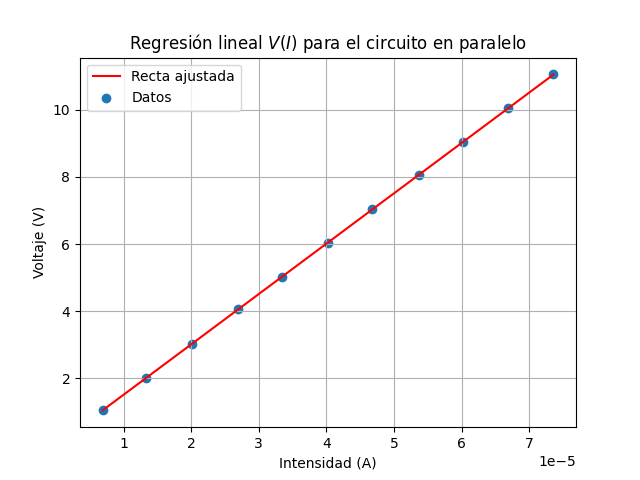
\includegraphics[width=14cm]{Figure_3M1.png}
    \end{center}
    \caption{Regresión lineal $V(I)$ del circuito en paralelo}
\end{figure}

\subsubsection{Resultados}

Como en los anteriores casos, podemos concluir que la medición experimental está en el intervalo dado por la $Ley$ $de$ $Ohm$ 
y la propagación de errores (\ref{eq:qwertr}) $[(1,495 \pm 0,001) \cdot 10^5 \subset ((1,499 - 0,056)\cdot 10^5,(1,499 + 0,056)\cdot 10^5)]$.
En lo que respecta a la verificación de (\ref{eq:intensidades}), observamos que la suma iguala en muchas ocasiones al valor del polímetor
, y cuando no lo hace presenta una variación muy pequeña. Una posible explicación es la disminución de incertidumbre al hacer la propagación de errores,
en otras palabras, es más fiable la medida de un circuito en paralelo.

\medskip

La mejor recta se ajusta con un $R^2 = 0.999997 \approx 1$ , entonces podemos concluir que los datos siguen una distribución lineal de parámetros
$a$ y $b$.
Respecto a la recta de regresión en sí, se observa otra vez el error de la coordenada en el origen $(a\neq 0)$, pero esta vez es 
mucho menor en comparación con la Sección \ref{sec:1.4}, y en todo caso, es menor a la desviación típica de la regresión. 
El error sistemático de antes ya no se aprecia de la misma manera puesto que es menor que los $0,04 \hspace{4pt}[V]$ apreciados.
En cuanto a la pendiente de la recta, $b=150176,4158\hspace{6pt}[\Omega]$ está en el intervalo teórico pero no en el experimental. Una
explicación es la tara que presenta el aparato de medida con el voltaje.

\subsection{\textbf{Conclusión}}

En esta práctica se ha verificado experimentalmente la $Ley$ $de$ $Ohm$ y sus consecuencias 
tanto en resistencias individuales como en circuitos en serie y
en paralelo mediante mediciones teóricas, directas e indirectas con y sin el polímetro.

Las resistencias medidas individualmente se encuentran dentro de los intervalos de tolerancia indicados
por el fabricante. Las estimaciones indirectas obtenidas mediante regresión lineal $V(I)$ presentan valores
de $R^2 \approx 1$, lo que confirma el carácter lineal de la $Ley$ $de$ $Ohm$. Las
pequeñas desviaciones observadas, como la no nulidad del término independiente, pueden atribuirse a errores
sistemáticos del instrumento y a errores aleatorios en las medidas.

En los circuitos en serie y en paralelo, las resistencias equivalentes obtenidas experimentalmente concuerdan,
dentro de la incertidumbre, con los valores teóricos calculados mediante propagación de errores. Asimismo,
se han comprobado experimentalmente la aditividad de los voltajes en serie y de las intensidades en paralelo,
en concordancia con el modelo teórico.

En conjunto, los resultados muestran una buena concordancia entre teoría y experimento, poniendo de
manifiesto la validez de las leyes fundamentales de la corriente continua y la importancia del análisis de
errores en la interpretación de datos experimentales.

\section{Práctica II (Corriente Alterna)}


\section{Anexo}
\subsection{Corriente Continua}

\begin{figure}[H]
    \centering
    \begin{subfigure}[b]{0.3\textwidth}
        \centering
        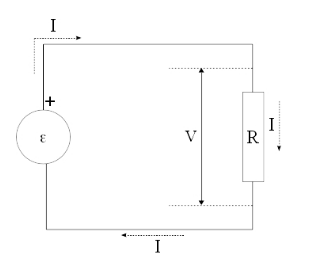
\includegraphics[width=\textwidth]{Resistencia.png}
        \caption{Circuito con una resistencia}
        \label{fig:Resistenciaa}
    \end{subfigure}
    \hfill
    \begin{subfigure}[b]{0.3\textwidth}
        \centering
        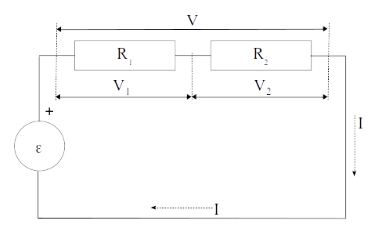
\includegraphics[width=\textwidth]{Serie.png}
        \caption{Circuito con dos resistencias en serie}
        \label{fig:Seriee}
    \end{subfigure}
    \hfill
    \begin{subfigure}[b]{0.3\textwidth}
        \centering
        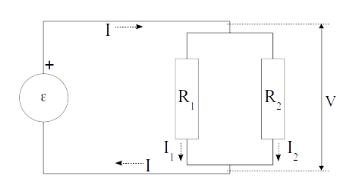
\includegraphics[width=\textwidth]{Paralelo.png}
        \caption{Circuito con dos resistencias en paralelo}
        \label{fig:Paraleloo}
    \end{subfigure}

    \caption{Circuitos de corriente continua}
    \label{fig:Corriente Continua}
\end{figure}

\subsection{Corriente Alterna}

\section{Bibliografía}
\printbibliography

\end{document}